\documentclass[10pt,journal]{IEEEtran}

\usepackage{amsmath,amssymb,amsfonts,mathtools,amsthm}
\usepackage{booktabs,array,multirow}
\usepackage{graphicx}
\usepackage{cite}
\usepackage{url}
\usepackage{enumitem}
\usepackage{microtype}
\usepackage{balance}
\graphicspath{{figures/}}
\usepackage[hidelinks]{hyperref}

\newtheorem{theorem}{Theorem}
\newtheorem{proposition}{Proposition}
\newtheorem{corollary}{Corollary}

\newcommand{\NetShield}{\textsc{NetShield}}
\newcommand{\Hnone}{\textsc{H-None}}
\newcommand{\Hsummary}{\textsc{H-Summary}}
\newcommand{\Hfull}{\textsc{H-Full}}
\newcommand{\IQPG}{\textsc{I-QPG}}
\newcommand{\CQPG}{\textsc{C-QPG}}
\newcommand{\SCQPG}{\textsc{S-CQPG}}
\newcommand{\CRFA}{\textsc{CRFA}}

\begin{document}

\title{\NetShield: Timely Evidence Feasibility under Shared Bottlenecks
for Multi-Probe Edge Intrusion Detection}

\author{
Nuonan~Ouyang,~\IEEEmembership{Member,~IEEE,}
Adrian~Shatte,
Zhigang~Lu,
Chao~Chen,~\IEEEmembership{Member,~IEEE,}
and~Wei~Xiang,~\IEEEmembership{Senior~Member,~IEEE}%
\thanks{\textit{(Corresponding author: Nuonan Ouyang.)}}%
\thanks{N. Ouyang and A. Shatte are with the College of Science and
Engineering, James Cook University, Bebegu Yumba Campus, Townsville,
QLD, Australia
(e-mail: nuonan.ouyang@my.jcu.edu.au;
adrian.shatte@jcu.edu.au).}%
\thanks{Z. Lu is with the School of Computer, Data and Mathematical
Sciences, Western Sydney University, Kingswood, NSW, Australia
(e-mail: z.lu@westernsydney.edu.au).}%
\thanks{C. Chen is with the College of Business and Law,
RMIT University, Melbourne, VIC, Australia
(e-mail: chao.chen@rmit.edu.au).}%
\thanks{W. Xiang is with La Trobe University,
Melbourne, VIC, Australia
(e-mail: w.xiang@latrobe.edu.au).}%
}

\markboth{IEEE Transactions on Networking---Submission Manuscript}%
{Ouyang \MakeLowercase{\textit{et al.}}:
Timely Evidence Feasibility under Shared Edge Bottlenecks}

\maketitle

% ============================================================
\begin{abstract}
Multi-probe edge intrusion detection couples evidence selection to network load: each probe can retain a decision locally, send a summary, or upload full evidence. NetShield characterizes this coupling through an exact coverage-conditioned byte-feasibility region, distinguishing same-round admission, finite-deadline service, and long-run load admissibility. Requiring every probe to remain remotely represented consumes capacity that could otherwise carry full evidence. In a three-probe configuration, this requirement costs one full-evidence slot at both low and middle budgets. A cyclic rotating admission controller attains the unrestricted byte frontier under ideal service while equalizing selection opportunities over time. Analysis also identifies a synchronized full/none cycle in independent queue-penalized control and gives a conditional rate-balance law, corroborated by phase-randomized software experiments. A 216-arm primary hardware campaign and a separately frozen 36-arm rotating-admission extension measure physical attainment of the analytical boundaries. The rotating controller realizes 91.7\%, 94.9\%, and 96.6\% of the low, middle, and high byte frontiers within one second after event creation. At the middle budget, timely full-core output is 0.6327 per generated event, compared with 0.2938 for session-matched summary-preserving admission; the nonconcurrent comparison is descriptive. All selected full results eventually return, locating the remaining shortfall in timing rather than evidence loss. Across both campaigns, 68,040 events and 74,340 reconstructed service rounds exhibit zero shared application-byte cap violations. These results quantify the price of per-round coverage and connect constructive admission guarantees to measured deadline attainment.
\end{abstract}

\begin{IEEEkeywords}
Internet of Things, intrusion detection, edge computing, admission control,
shared bottleneck, evidence scheduling, latency SLO, queue-aware control.
\end{IEEEkeywords}

% ============================================================
\section{Introduction}
\label{sec:introduction}

Edge intrusion detection increasingly combines local inference with remote
evidence handling. A probe may retain a decision locally, emit a compact
summary, or upload richer evidence for core-side execution and correlation.
These actions differ not only in security utility but also in the number of
bytes injected into a shared service. Evidence generation is therefore an
\emph{endogenous networking decision}: the controller chooses the offered
load before the bottleneck serves it.

This distinction matters when several probes act concurrently. If three
probes each request a 128~KiB full upload, the aggregate request is
393,216~B. Under a service budget smaller than that amount, every local
request may be reasonable in isolation while the joint tuple is infeasible.
The relevant question is not merely whether the detector runs, but how much
remote-evidence coverage and full-evidence richness can be delivered within
a response horizon.

Recent work on remote inference explicitly couples communication timing,
feature freshness, and inference quality~\cite{shisher2024timely,
ari2026goal}, while modern edge systems expose request scheduling and
admission as first-class resource-allocation problems~\cite{zhao2024cur,
hao2024edgetimer,li2025oacr2}. Security systems likewise show that collecting
and transporting the data needed for detection can itself become a
bottleneck~\cite{mirnajafizadeh2024isdc,oqaily2024chainpatrol}. \NetShield{}
connects these observations in a multi-probe security setting by making the
evidence action itself part of the network load model.

Shared feedback creates a second issue: synchronization. When identical
independent probes observe the same queue states at synchronized decision
epochs, they can repeatedly choose the same actions. In the tested middle
budget, this creates a full-upload/no-upload cycle. Separating this mechanism
from shared-capacity admission is essential to understanding which controller
realizes the feasible evidence allocation.

The paper asks four questions:
\begin{itemize}[leftmargin=1.25em]
\item \textbf{RQ1---Feasibility and the price of coverage:}
What full-evidence throughput is byte-feasible, and what is lost when every
probe must retain remote evidence in every round?
\item \textbf{RQ2---Controller realization and synchronization:}
How do coordinated and independent controllers occupy the feasible region,
and when does local queue feedback create synchronized limit cycles?
\item \textbf{RQ3---Physical timing residual:}
Once a byte allocation is feasible, how do orchestration and wireless timing
affect post-release and schedule-inclusive service attainment?
\item \textbf{RQ4---Scaling and reproducibility:}
Do the analytical boundaries hold as $n$ changes, and can the hardware result
chain be reconstructed from occurrence-level evidence?
\end{itemize}

The paper makes three contributions.

\textbf{1) Quantifying the price of per-round coverage.}
We derive the exact coverage-conditioned region and its unrestricted
full-evidence frontier. Their integer difference measures how many full
uploads are exchanged for universal remote representation. A hierarchy of
same-round, finite-deadline, and long-run feasibility identifies the service
condition each boundary addresses.

\textbf{2) Constructing admission and explaining controller dynamics.}
Cyclic rotating full admission (\CRFA{}) reaches the unrestricted byte
frontier under ideal service and equalizes selection opportunities. For
independent queue-penalized control, we identify the synchronized full/none
orbit and derive a conditional rate-balance law for the saturated reduced
regime. Phase-randomized software conforms to the predicted request rates.

\textbf{3) Measuring frontier attainment on physical hardware.}
A 216-arm primary campaign and a separately frozen 36-arm \CRFA{} extension
use three heterogeneous Raspberry Pi probes. The extension realizes 91.7\%,
94.9\%, and 96.6\% of the low/mid/high byte frontier within the 1-s
post-release service SLO. Occurrence-level reconstruction separates
byte-feasible selection from result-return timing across both campaigns.

\NetShield{} studies evidence admission and service feasibility with a fixed
detector/action set, connecting coverage requirements, controller dynamics,
and measured deadline attainment.

\section{Related Work}
\label{sec:related}

\subsection{IoT Intrusion Detection and Generalization}
Lightweight IoT IDS research has produced compact anomaly detectors, device
fingerprints, and online pipelines, including SVELTE, IoT Sentinel, N-BaIoT,
and Kitsune~\cite{raza2013svelte,miettinen2017iotsentinel,
meidan2018nbaiot,mirsky2018kitsune}. More recent work addresses lightweight
open-set detection for previously unseen IIoT attacks~\cite{yang2025openset}.
These systems primarily optimize the detector. \NetShield{} instead freezes
the detector/evidence action set and studies whether the resulting evidence
requests can be sustained jointly. Deployment generalization is a separate detector-evaluation question
~\cite{sommer2010closedworld}; Section~\ref{sec:limitations} describes the
frozen replay used here.

\subsection{Security Data Collection and Evidence Overhead}
Recent security systems make the cost of acquiring evidence explicit. ISDC
prioritizes network-defense data collection under constrained in-network
resources~\cite{mirnajafizadeh2024isdc}, while ChainPatrol trades attack
visibility against traffic and delay overhead for service-function-chain
verification~\cite{oqaily2024chainpatrol}. These works motivate treating
security evidence as a resource-consuming network object rather than a free
by-product of detection. Our control point is complementary: the runtime
action determines both how many probes remain remotely represented and how
rich their evidence is before shared-service admission.

\subsection{Edge Scheduling and Admission Control}
Mobile/edge computing studies placement and offloading under latency,
bandwidth, and energy constraints~\cite{mao2017mec,mach2017mec}. Recent
systems make scheduling and admission more explicit: Cur-CoEdge coordinates
edge-cloud request scheduling~\cite{zhao2024cur}, EdgeTimer adapts scheduling
timescales in MEC~\cite{hao2024edgetimer}, and OACR$^2$ jointly controls
online admission and resource reservation for network slices
~\cite{li2025oacr2}. Classical fair queueing and GPS instead determine how a
bottleneck serves traffic after it has entered queues~\cite{demers1989fair,
parekh1993gps}. \NetShield{} combines evidence admission with an explicit
per-round representation constraint: the budget must account for both the
summary baseline and the incremental cost of full evidence.

\subsection{Collaborative Perception and Learning Uploads}
Multi-vehicle perception systems jointly choose what sensor data to share
and how to deliver it. EMP partitions point clouds and coordinates uploads
to an edge server~\cite{zhang2021emp}; Harbor combines vehicle-to-vehicle
relaying with edge-assisted processing under heterogeneous connectivity
~\cite{zhu2024harbor}. In federated learning, FedCS selects clients using
communication and computation constraints to aggregate more updates within
a round~\cite{nishio2019fedcs}. These systems already couple participation
or data volume to shared resources. The distinctive object in \NetShield{}
is the integer cost of requiring every probe to retain remote evidence,
together with a constructive alternative that exchanges same-round coverage
for equal full-evidence opportunities over time. Perception accuracy and
learning convergence are different objectives from the timely evidence
output measured here.

\subsection{Queue-Aware Network Control}
Queue-aware scheduling and Lyapunov drift-plus-penalty provide a foundation
for balancing utility against backlog~\cite{tassiulas1992,neely2010}.
Recent ToN work also combines Lyapunov-style queue scheduling with online
learning under non-stationary conditions~\cite{huang2024lyapunovbandit}.
Here, a frozen finite-action queue penalty provides a tractable case for
studying synchronization. We analyze its stated score in~\eqref{eq:qpg}
and label the implementations independent queue-penalized greedy (\IQPG),
coordinated QPG (\CQPG), and safety-filtered coordinated QPG (\SCQPG).

\subsection{Timely Remote Inference and Serving}
Prediction-serving systems expose latency-resource trade-offs through
batching, provisioning, and execution control. Clipper, Nexus, Clockwork, and
InferLine are representative systems~\cite{crankshaw2017clipper,
shen2019nexus,gujarati2020clockwork,crankshaw2020inferline}; SuperServe
extends this line to fine-grained serving under unpredictable workloads
~\cite{khare2025superserve}. Networking work on remote inference instead
optimizes feature freshness, packet length, or transmission timing
~\cite{shisher2024timely,ari2026goal}. Age-of-information scheduling also
jointly considers freshness and minimum throughput~\cite{kadota2019aoi},
while timely-throughput theory treats deadlines, delivery ratios, and
channel reliability as joint feasibility requirements~\cite{hou2009qos}.
Thus neither upload selection nor timeliness alone distinguishes this work.
\NetShield{} isolates the additional cost of per-round remote representation
and measures timely full-evidence output against the resulting integer
frontier. Its rotation bounds selection gaps; an information-age guarantee
would additionally require successful-delivery timing.

The finite-deadline layer specializes the classical preemptive
processor-demand feasibility criterion~\cite{baruah1990feasibility} to the
common-deadline byte-service model. This established criterion supplies the
connection between same-round admission and average load; the new evidence
characterization concerns the coverage-conditioned allocation and its
physical realization.

\subsection{Runtime Safety Filters and Prior Work}
Runtime shields and predictive safety filters separate policy choice from
hard enforcement~\cite{alshiekh2018shielding,wabersich2021filter}. We retain
that architecture as an optional local-feasibility interface. Its relation
to shared-capacity admission is evaluated separately in the intervention
audit (Section~\ref{sec:results}).

Our prior ACISP 2026 Systematization of Knowledge surveyed telemetry-aware
runtime assurance for always-on on-device IDS and presented TQS-IDS as a
design template~\cite{ouyang2026sok}. It did not implement the shared-
bottleneck formulation, the queue-penalized controllers, the event contract,
or the three-Pi hardware campaign studied here.

\section{System Model and Feasibility Analysis}
\label{sec:model}

\subsection{Shared Evidence Service}
Table~\ref{tab:notation} collects the core notation; the Supplementary
Notation Index additionally lists timing and planning symbols. Consider
$n$ edge probes sharing an enforced application-payload service budget
$C(t)$ bytes in coordination round $t$. A coordination round is the shared
allocator's accounting step. This budget is distinct from the physical
link rate; wireless, processing, and orchestration delays are measured
separately through event timestamps. We write $C$ for a constant budget.
Throughout, MB denotes $10^6$ bytes, while KiB and MiB denote $2^{10}$ and
$2^{20}$ bytes, respectively.

\begin{table}[t]
\centering
\caption{Core notation. Counts refer to a single round unless stated.}
\label{tab:notation}
\small
\renewcommand{\arraystretch}{1.08}
\begin{tabular}{@{}p{0.30\columnwidth}p{0.64\columnwidth}@{}}
\toprule
Symbol & Meaning \\
\midrule
$n;\ m,k$ & Probes; remotely represented and full-evidence counts ($k\leq m\leq n$). \\
$B,S;\ C$ & Full and summary bytes; shared bytes per round. \\
$\rho,\sigma$ & Normalized capacity $C/(nB)$ and summary ratio $S/B$. \\
$r,f$ & Coverage $m/n$ and full-evidence fraction $k/n$. \\
$K_{\rm full}^{\max},K_{\rm all}^{\max}$ & Full counts without/with universal remote coverage; $K=K_{\rm full}^{\max}$. \\
$Q_i(t),g_i(t)$ & Queued bytes and service grant for probe $i$. \\
$a;\ b(a),u(a),v$ & Action; payload, utility, and queue-score weight. \\
$A_t,D$ & Aggregate admitted bytes; relative deadline in rounds. \\
$p;\ \mathcal S_t$ & Long-run full-request fraction; rotating selection set. \\
\bottomrule
\end{tabular}
\end{table}
 Probe $i$ has evidence queue $Q_i(t)$ and
chooses an admitted action $a_i(t)$ with payload $b(a_i)$. The common service
grants $g_i(t)$ satisfy
\begin{equation}
g_i(t)\geq0,\qquad \sum_{i=1}^{n}g_i(t)\leq C(t),
\label{eq:cap}
\end{equation}
and the queue evolves as
\begin{equation}
Q_i(t+1)=\left[Q_i(t)+b(a_i(t))-g_i(t)\right]^+.
\label{eq:queue}
\end{equation}

\subsection{Frozen Action Lattice}
The implementation exposes ten frozen actions spanning light, medium, and
heavy detector execution and evidence levels from no upload to full core-side
evidence. Table~\ref{tab:actions} lists the frozen payload and utility fields.

\begin{table}[t]
\centering
\caption{Frozen action payloads and utility scores.}
\label{tab:actions}
\scriptsize
\begin{tabular}{@{}lrr@{}}
\toprule
Action & Payload (B) & Utility \\
\midrule
L-NONE    & 0      & 0.758501 \\
L-ALERT   & 256    & 0.825168 \\
L-SUMMARY & 4,096  & 0.891835 \\
M-NONE    & 0      & 0.766968 \\
M-ALERT   & 256    & 0.833635 \\
M-SUMMARY & 8,192  & 0.900302 \\
H-NONE    & 0      & 0.768378 \\
H-ALERT   & 256    & 0.835044 \\
H-SUMMARY & 16,384 & 0.901711 \\
H-FULL    & 131,072& 0.968378 \\
\bottomrule
\end{tabular}
\end{table}

The coordinated regimes eventually operate on the \Hsummary--\Hfull{}
edge of this lattice, which admits an exact coverage--richness boundary.

\subsection{One-Round Coverage--Richness Region}
Let $m\leq n$ probes retain remotely delivered evidence in a round. Among
them, let $k\leq m$ send full evidence of size $B$; the other $m-k$ send
summaries of size $S$, where $0<S<B$. The remaining $n-m$ probes generate no
remote evidence.

\begin{theorem}[Coverage-conditioned one-round feasibility]
\label{thm:frontier}
A $(k,m)$ allocation is byte-feasible within one idealized service round if
and only if
\begin{equation}
kB+(m-k)S\leq C.
\label{eq:feasible}
\end{equation}
For fixed $m$, if $C\geq mS$, the maximum feasible full-evidence count is
\begin{equation}
k^\star(C,m)=
\min\left\{m,\left\lfloor\frac{C-mS}{B-S}\right\rfloor\right\}.
\label{eq:kstar}
\end{equation}
If $C<mS$, no allocation preserving remote evidence for all $m$ probes is
feasible.
\end{theorem}

\begin{proof}
The payload is $mS+k(B-S)$. If $C<mS$, even the all-summary allocation is
infeasible. Otherwise, since $B-S>0$, feasibility is equivalent to
$k(B-S)\leq C-mS$; the largest feasible integer $k$ is therefore
\eqref{eq:kstar}, clipped by $m$.
\end{proof}

Define $\rho=C/(nB)$, $\sigma=S/B$, $r=m/n$, and $f=k/n$. Ignoring
finite-$n$ granularity,~\eqref{eq:feasible} becomes
\begin{equation}
\boxed{\sigma r+(1-\sigma)f\leq\rho}.
\label{eq:frontier}
\end{equation}
This continuous relaxation separates the capacity spent on remote coverage
from that spent upgrading summaries to full evidence. The integer boundary
fixes the feasible set independently of the controller: the subsequent
analysis asks which point a controller selects and how much of that
byte-feasible allocation meets the physical service horizon.

\begin{corollary}[Full-evidence byte frontier and price of coverage]
\label{cor:fullfrontier}
If non-selected probes may send no remote evidence, the maximum number of
full-evidence probes whose bytes can fit in one idealized round is
\begin{equation}
K_{\rm full}^{\max}(C)
=\min\left\{n,\left\lfloor\frac{C}{B}\right\rfloor\right\}.
\label{eq:kfullmax}
\end{equation}
If every probe must remain remotely represented, the maximum is
\begin{equation}
K_{\rm all}^{\max}(C)
=\left[\left\lfloor\frac{C-nS}{B-S}\right\rfloor\right]_0^n,
\label{eq:kallmax}
\end{equation}
provided $C\geq nS$. The full-slot price of universal per-round remote
coverage is
\begin{equation}
\Pi_{\rm cov}(C)=K_{\rm full}^{\max}(C)-K_{\rm all}^{\max}(C).
\label{eq:coverageprice}
\end{equation}
\end{corollary}

\begin{proof}
For any feasible pair, $m\geq k$ and $S>0$. For fixed $k$, payload is
minimized by $m=k$, which costs $kB$. Thus no allocation can contain more than
$\lfloor C/B\rfloor$ full requests, and choosing $m=k$ attains that count.
Equation~\eqref{eq:kallmax} is Theorem~\ref{thm:frontier} with $m=n$.
\end{proof}

The quantity $K_{\rm full}^{\max}/n$ is a one-round \emph{byte-completion}
frontier. It is not by itself a physical 1-s result-return guarantee because
core processing, wireless timing, and orchestration occur after or alongside
byte service.

\subsection{Three Feasibility Layers}
The one-round region is the strongest of three useful service notions. The
following specialization of preemptive processor-demand feasibility
~\cite{baruah1990feasibility} connects these layers. Let
$A_t$ denote total admitted bytes released at the beginning of round $t$, and
consider an ideal preemptive fluid server of capacity $C$ bytes per round.

\begin{proposition}[Same-round, finite-deadline, and load feasibility]
\label{prop:layers}
For a common relative deadline of $D\geq1$ rounds, a necessary and sufficient
demand condition under the ideal fluid/EDF model is
\begin{equation}
\sum_{\tau=s}^{t} A_\tau
\leq C(t-s+D),\qquad \forall~s\leq t.
\label{eq:demandbound}
\end{equation}
When $D=1$, this reduces to same-round feasibility $A_t\leq C$ for every
$t$. Any finite-$D$ feasible sequence also satisfies the long-run load
condition
\begin{equation}
\limsup_{T\rightarrow\infty}
\frac{1}{T}\sum_{t=1}^{T}A_t\leq C.
\label{eq:rateadm}
\end{equation}
Thus, for finite $D$,
\begin{equation}
\mathcal F_{\rm same}
\subseteq\mathcal F_D
\subseteq\mathcal F_{\rm rate}.
\label{eq:layers}
\end{equation}
\end{proposition}

\begin{proof}
A job released in round $\tau$ has deadline $\tau+D-1$. The processor-
demand criterion~\cite{baruah1990feasibility} for a preemptive single fluid
server requires that, for any
service interval, the work whose release times and deadlines both fall inside
that interval not exceed available service. Re-indexing the interval gives
~\eqref{eq:demandbound}. Setting $D=1$ yields per-round feasibility. Finally,
using $s=1$ and dividing~\eqref{eq:demandbound} by $T$ gives
$T^{-1}\sum_{t=1}^T A_t\leq C[1+(D-1)/T]$, whose limsup is~\eqref{eq:rateadm}.
\end{proof}

Equation~\eqref{eq:rateadm} is a load-admissibility condition, not a claim
that an arbitrary burst process with mean exactly $C$ has bounded delay.
Standard queue-stability conclusions require additional arrival assumptions
and typically strict slack~\cite{tassiulas1992,neely2010}.

\subsection{Deterministic Overload Growth}
\begin{proposition}[Fixed-full overload law]
\label{prop:overload}
If every probe generates $B$ bytes per generation round, the initial queues
are empty, aggregate service is work conserving, and $C<nB$, then after $T$
generation rounds
\begin{equation}
Q_\Sigma(T)=T(nB-C).
\label{eq:overload}
\end{equation}
Under symmetric fair service, per-probe backlog is approximately
$T(B-C/n)$ up to integer-grant rounding.
\end{proposition}
\begin{proof}
Each round adds $nB$ bytes. Work-conserving service removes
$\min\{Q_\Sigma(t)+nB,C\}=C$, since $nB>C$ even when the queue is empty.
Thus backlog grows by exactly $nB-C$ each round; summing from the empty
initial state yields~\eqref{eq:overload}.
\end{proof}

\subsection{Independent Queue-Penalized Selection}
The frozen independent policy maximizes the score
\begin{equation}
\psi_i(a,t)=v u(a)-Q_i(t)b(a)/10^6,
\label{eq:qpg}
\end{equation}
where $u(a)$ is the frozen utility in Table~\ref{tab:actions}, $v$ weights
utility against the queue--payload penalty, and both $Q_i(t)$ and $b(a)$
are in bytes. At $v=1$, a positive-payload action $a$ can beat \Hnone{}
only while
\begin{equation}
Q_i<q_a=\frac{[u(a)-u(\Hnone)]10^6}{b(a)}.
\label{eq:threshold}
\end{equation}
For the relevant actions, $q_{\Hfull}\approx1.526$~B,
$q_{\Hsummary}\approx8.138$~B, and the largest threshold over any
positive-payload action is about 260.4~B (H-ALERT). At mid capacity, a
synchronized three-probe full round leaves
$q^+=B-2B/3=B/3\approx43{,}691$~B (42.7~KiB) per probe.

\begin{proposition}[Symmetry-induced period-two orbit]
\label{prop:cycle}
Suppose synchronized probes have identical state and empty queues, choose
\Hfull{} when $Q_i=0$, and a synchronized full round leaves residual $q^+$.
If $q^+>\max_{a:b(a)>0}q_a$ and a zero-payload round can drain $q^+$, then
the controller enters the orbit
$\Hfull\rightarrow\Hnone\rightarrow\Hfull\rightarrow\cdots$.
\end{proposition}
\begin{proof}
After the full round, every positive-payload action scores below \Hnone{}.
The next zero-payload round drains the residual and restores the empty state,
so symmetry makes all probes repeat the same sequence.
\end{proof}

\begin{proposition}[Rate balance in the reduced desynchronized regime]
\label{prop:prho}
Consider the reduced regime in which each probe receives one request
opportunity per round and emits either $B$ bytes (\Hfull) or zero bytes
(\Hnone). Let $p$ be the long-run fraction of request opportunities that
emit $B$. Aggregate rate stability implies
\begin{equation}
p\leq \min\left(1,\frac{C}{nB}\right)=\min(1,\rho).
\label{eq:prhobound}
\end{equation}
If $C<nB$ and the shared server is asymptotically saturated, equality holds.
If $C\geq nB$ and an unbacklogged probe requests full evidence at every
opportunity, then $p=1$. Hence the saturated reduced regime has
\begin{equation}
p^\star=\min(1,\rho).
\label{eq:prho}
\end{equation}
\end{proposition}
\begin{proof}
Queue conservation over $T$ rounds gives
$Q_\Sigma(T)=Q_\Sigma(0)+Bn pT-S(T)+o(T)$. Rate stability and the service
bound $S(T)/T\leq C+o(1)$ imply $npB\leq C$, together with the trivial
$p\leq1$. When $C<nB$ and $S(T)/T\rightarrow C$, rate stability forces
$npB=C$. When $C\geq nB$, requesting at every unbacklogged opportunity gives
$p=1$ and remains load-feasible.
\end{proof}

Equation~\eqref{eq:prho} characterizes the saturated, rate-stable reduced
regime specified above.

\subsection{A Fair Construction at the Full-Evidence Frontier}
Let $K=K_{\rm full}^{\max}(C)$. A simple cyclic construction selects exactly
$K$ probes for \Hfull{} in each round and assigns \Hnone{} to the rest.

\begin{proposition}[Cyclic rotating full admission]
\label{prop:rotation}
Index probes modulo $n$ and define
\begin{equation}
\mathcal S_t=\{(tK+j)\bmod n: j=0,\ldots,K-1\}.
\label{eq:rotation}
\end{equation}
Then every round is one-round byte-feasible and attains
$K_{\rm full}^{\max}$. The selection pattern has period
\begin{equation}
T_{\rm fair}=\frac{n}{\gcd(n,K)},
\label{eq:fairperiod}
\end{equation}
and each probe is selected exactly $K/\gcd(n,K)$ times per period.
\end{proposition}
\begin{proof}
Each round injects exactly $KB\leq C$. Advancing the starting index by $K$
returns to the initial residue after $n/\gcd(n,K)$ rounds. Across that
period there are $KT_{\rm fair}$ selection slots distributed symmetrically
over $n$ residues, giving $K/\gcd(n,K)$ selections per probe.
\end{proof}

This construction converts per-round coverage into temporal fairness: at mid
capacity with $n=3$ and $K=2$, the three-round sequence can be
$\{P1,P2\}\rightarrow\{P3,P1\}\rightarrow\{P2,P3\}$, so every probe
receives two full-evidence opportunities per three rounds. We first verify
this schedule under idealized service accounting and then test the same
construction in a separately frozen physical extension described in
Section~\ref{sec:method}.

\subsection{Joint Admission and Optional Safety Filtering}
\CQPG{} first obtains per-probe queue-penalized requests and monotonically
reduces simultaneous requests until the common budget is satisfied.
\SCQPG{} adds a local safety filter before the same joint admission stage.
Network byte feasibility follows from joint admission. In the hardware
campaign, low-capacity safety filtering and ordinary shared-capacity
admission reach the same final summary mix; Section~\ref{sec:results}
reports the intervention audit.

\section{Experimental Methodology}
\label{sec:method}

\subsection{Physical Testbed and Workload}
The testbed uses three physical probes: P1 is a Raspberry Pi~5, P2 a
Raspberry Pi~4B, and P3 a Raspberry Pi~3B+. Probe-to-core experiment traffic
uses Wi-Fi, and the edge core executes the heavy core path for \Hfull{}
events.

The workload is a frozen feature-vector replay derived from
CICIoT2023~\cite{neto2023ciciot}, not packet replay. Detector models, feature
order, action profiles, window plans, and formal configuration are frozen
before the primary campaign. Each arm uses five warm-up rounds followed by 90
measured event occurrences per probe, with up to 200 drain rounds. The primary
matrix is
\[
12~\text{sessions}\times6~\text{methods}\times3~\text{capacities}
=216~\text{arms},
\]
giving 648 device-runs and 58,320 measured events. The rotating extension
reuses the same three probes, action definitions, session/workload identities,
and measured-window contract, but is archived as a separate campaign.

\subsection{Shared Service Budgets}
The formal application-byte budgets are shown in Table~\ref{tab:capacity}.
Because $B=128$~KiB, they correspond to one, two, or three full-evidence byte
equivalents.
\begin{table}[t]
\centering
\caption{Application-service budgets.}
\label{tab:capacity}
\small
\begin{tabular}{@{}lrr@{}}
\toprule
Regime & Budget (B/round) & Full equivalents \\
\midrule
Low  & 131,072 & 1 \\
Mid  & 262,144 & 2 \\
High & 393,216 & 3 \\
\bottomrule
\end{tabular}
\end{table}

\subsection{Hardware Methods}
Table~\ref{tab:methods} summarizes the primary hardware methods.
\begin{table*}[t]
\centering
\caption{Hardware methods. Historical artifact identifiers are retained only
in the reproducibility package, not as algorithmic claims.}
\label{tab:methods}
\small
\begin{tabular}{@{}cll@{}}
\toprule
ID & Paper name & Runtime semantics \\
\midrule
A & Fixed local & Always \Hnone; no application evidence upload. \\
B & Fixed summary & Always \Hsummary. \\
C & Fixed full & Always \Hfull; no joint pre-admission. \\
D & \IQPG & Per-probe queue-penalized selection; no joint admission. \\
E & \CQPG & Queue-penalized requests plus joint shared-capacity admission. \\
F & \SCQPG & Local safety filtering followed by the same joint admission. \\
\bottomrule
\end{tabular}
\end{table*}

\subsection{Separately Frozen Rotating-Admission Extension}
\label{sec:crfa_method}
After the analytical frontier and the primary campaign had been frozen, we
executed a separate hardware extension using cyclic rotating full admission
(\CRFA{}). In each measured round, \CRFA{} admits exactly
$K_{\rm full}^{\max}(C)$ probes with \Hfull{} and assigns \Hnone{} to the
remaining probes; admitted identities follow the cyclic schedule in
Proposition~\ref{prop:rotation}. The extension therefore tests the
unrestricted full-evidence frontier rather than another utility optimizer.

The extension uses the same 12 session/workload identities and three service
budgets, giving
\[
12~\text{sessions}\times3~\text{capacities}=36~\text{accepted arms}.
\]
The frozen protocol retains the same five warm-up rounds, 90 measured
occurrences per probe, and drain rules as the primary campaign. The resulting
hardware evidence contains 9,720 measured occurrences and 10,620 reconstructed
shared-service rounds.

Across execution, 55 attempts were indexed. Nineteen were excluded in full
under pre-specified infrastructure/data-integrity rules, predominantly SSH
transport or pre-arm hardware-gate failures; all excluded attempts remain in
the attempt index. Timing outcomes were never used as acceptance criteria and
partial attempts were not stitched into accepted arms. The 36 accepted arms
pass event-identity, action/payload-identity, final-drain, raw-reconstruction,
and shared-cap gates, with zero shared-cap violations.

For descriptive comparison with the primary \CQPG{} results, \CRFA{} arms are
matched by the frozen session/workload identifier. Because the extension was
executed separately rather than as a concurrent randomized A/B trial, paired
session-bootstrap intervals are interpreted as matched descriptive timing
contrasts rather than as causal treatment intervals.

\subsection{Event-Level Metric Authority}
The occurrence-level event ledger is the scientific source of truth. Each
admitted event retains an immutable execution contract specifying whether its
result is local or core-dependent and what evidence transfer is required.
For a core-required event $e$, post-release latency is
\begin{equation}
L_{\mathrm{post}}(e)=t_{\mathrm{return}}(e)-t_{\mathrm{created}}(e),
\label{eq:postlat}
\end{equation}
and the primary service SLO is $L_{\mathrm{post}}\leq1$~s. The
schedule-inclusive sensitivity instead uses
\begin{equation}
L_{\mathrm{nom}}(e)=t_{\mathrm{return}}(e)-t_{\mathrm{scheduled}}(e).
\label{eq:nomlat}
\end{equation}
Missing results remain in the denominator and are not counted as on time.

The primary service quantities are core-required fraction, result-return
coverage, post-release on-time core-result coverage, conditional on-time rate
among core-required events, generated application payload, and queue
occupancy. Classifier correctness is not multiplied into the main service
metric because correctness is constant on the scored formal replay
occurrences.

\subsection{Statistical Reporting}
Action composition, core-required fractions, exact byte totals, analytical
queue growth, and admission counts are deterministic under a frozen plan and
are reported exactly without confidence intervals. Timing-derived quantities
vary across physical sessions; the session is the independent replicate
($n=12$). Paired session-bootstrap intervals are used only as descriptive
timing contrasts. For the separately executed \CRFA{} extension, matching is
by frozen session/workload identity rather than concurrent wall-clock
execution.

\subsection{Offline Sensitivity and Conformance Analyses}
Five read-only analyses complement the hardware campaign without modifying
its accepted raw evidence.

\textbf{Queue-weight sensitivity.}
The exact frozen \IQPG{} objective and allocator are replayed over 12 formal
seeds for
\begin{multline*}
v\in\{1,3,10,30,100,168,300,1000,\\
3000,10000,30000,100000\}.
\end{multline*}
The $v=1$ replay must reproduce the hardware action mix, payload, core
fraction, and sampled maximum queue before the sweep is accepted.

\textbf{Phase-randomized independent control.}
Twenty fixed seeds assign each probe an independent initial phase in $[0,1)$~s.
Each probe observes only its own queue; no action/queue exchange and no joint
admission are introduced. This is a discrete-event software sensitivity, not
a hardware measurement.

\textbf{Schedule-anchor reconstruction.}
Both~\eqref{eq:postlat} and~\eqref{eq:nomlat} are reconstructed directly
from accepted hardware timestamps for all 648 session/method/capacity/device
cells.

\textbf{Probe-count conformance.}
A discrete-event simulator evaluates $n\in\{3,8,16,32\}$ and
$\rho\in\{1/3,1/2,2/3,3/4,1\}$ for the summary-preserving $m=n$ case.
This tests the integer boundary only; it is not a 32-node hardware experiment.

\textbf{Rotating-frontier conformance.}
Using the same 1-ms service accounting as the phase study, the cyclic
construction in Proposition~\ref{prop:rotation} is checked at all three
capacities. This software check verifies the action/count semantics
independently of the later \CRFA{} hardware extension.

\section{Results}
\label{sec:results}

\subsection{RQ1: Universal Per-Round Coverage Has a Quantifiable Byte Cost}
For the physical testbed,
$n=3$, $B=128$~KiB, and $S=16$~KiB, so $\sigma=1/8$.
Figure~\ref{fig:frontier} shows the relaxed byte-budget boundary.
When all probes retain remote evidence ($m=n$), the coordinated policies
occupy the exact 0/1/3-full operating points predicted by
Theorem~\ref{thm:frontier} in every primary-campaign hardware session.

\begin{figure*}[t]
\centering
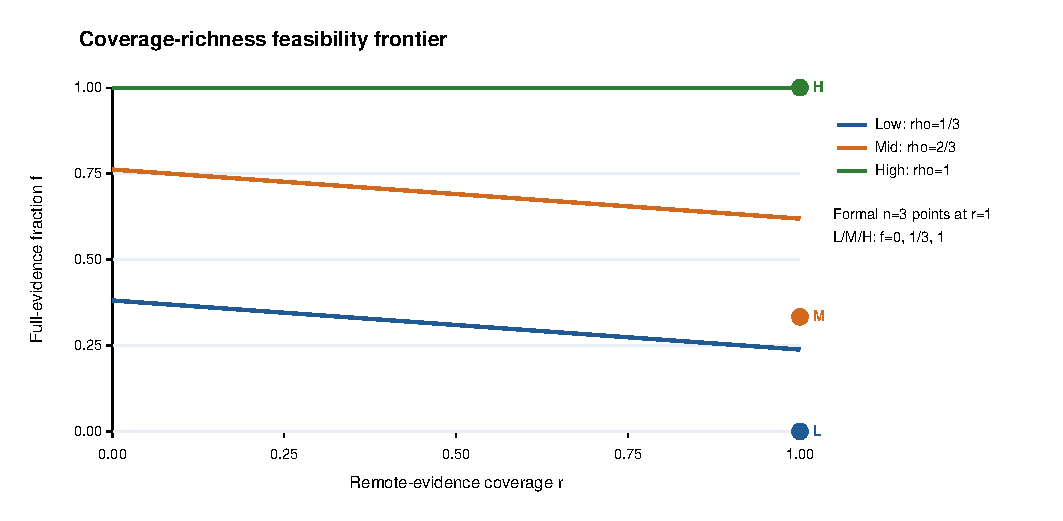
\includegraphics[width=0.92\textwidth]{fig1_feasibility_frontier.pdf}
\caption{Relaxed coverage--richness byte-budget lines; admissible points
also satisfy $0\leq f\leq r\leq1$. Markers are the physical $n=3$
summary-preserving coordinated operating points.}
\label{fig:frontier}
\end{figure*}

Corollary~\ref{cor:fullfrontier} gives the unrestricted comparison in
Table~\ref{tab:coverageprice} and Fig.~\ref{fig:coverageprice}. If non-selected probes may send no remote
evidence, the one-round byte frontier is 1/2/3 full probes at low/mid/high
capacity. Requiring all three probes to remain remotely represented reduces
this to 0/1/3. Universal per-round coverage therefore costs one full-evidence
slot at the two binding capacities and no slot at high capacity.

\begin{table}[t]
\centering
\caption{One-round full-evidence byte frontier and price of universal
per-round remote coverage.}
\label{tab:coverageprice}
\small
\begin{tabular}{@{}lrrrr@{}}\toprule
Regime & $K_{\rm full}^{\max}$ & $K_{\rm all}^{\max}$ & Price & $f_{\rm byte}^{\max}$ \\
\midrule
Low & 1 & 0 & 1 & 0.333 \\
Mid & 2 & 1 & 1 & 0.667 \\
High & 3 & 3 & 0 & 1.000 \\
\bottomrule\end{tabular}

\end{table}

\begin{figure}[t]
\centering
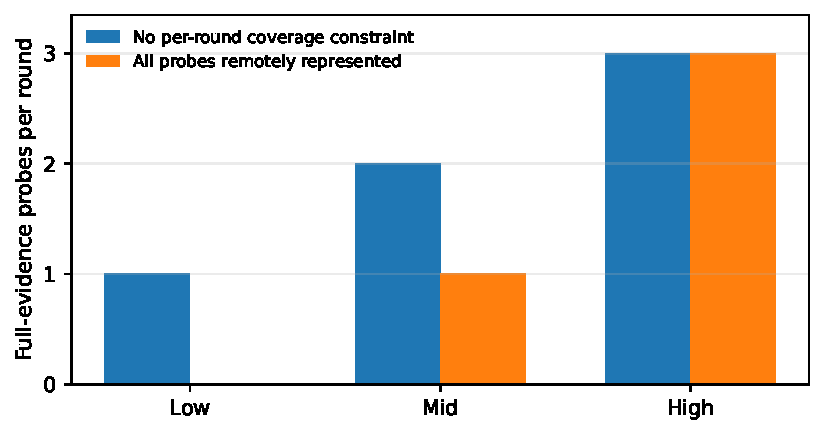
\includegraphics[width=\columnwidth]{fig2_coverage_price.pdf}
\caption{Maximum one-round full-evidence count with and without the
constraint that every probe remains remotely represented.}
\label{fig:coverageprice}
\end{figure}

The separately frozen \CRFA{} extension provides a constructive physical
test of the unrestricted operating points. In every measured service round,
the admitted action pattern is exactly one, two, or three \Hfull{} actions
at low, mid, and high capacity, with \Hnone{} on non-selected probes. The
aggregate measured application payload therefore equals the corresponding
131,072/262,144/393,216-B budget in every measured round; all pre-service
queues are zero and no shared-cap violation occurs.

The more informative result is how much of the byte frontier survives the
1-s post-release service SLO. Table~\ref{tab:crfa} and Fig.~\ref{fig:crfa}
report timely full-core results on the common generated-event denominator. \CRFA{} achieves 0.3056,
0.6327, and 0.9660 at low, mid, and high capacity, equal to 91.7\%, 94.9\%,
and 96.6\% of the unrestricted byte frontier. All selected full-evidence
events eventually return a core result; the remaining gap is therefore
deadline lateness, not missing evidence.

\begin{table*}[t]
\centering
\caption{\CRFA{} hardware attainment of the unrestricted frontier. Timely
full is on-time full-core results divided by all generated events. C-QPG is
the matched summary-preserving hardware comparator. $\Delta$ is
CRFA--C-QPG; intervals are descriptive 95\% paired session-bootstrap
intervals over the 12 frozen session/workload identities.}
\label{tab:crfa}
\scriptsize
\begin{tabular}{@{}lrrrrr@{}}
\toprule
Capacity & Byte frontier & C-QPG & CRFA & Attainment & $\Delta$ CRFA--C-QPG (95\% CI) \\
\midrule
Low & 0.3333 & 0.0000 & 0.3056 & 0.9167 & +0.3056 [+0.3015, +0.3093] \\
Mid & 0.6667 & 0.2938 & 0.6327 & 0.9491 & +0.3389 [+0.3306, +0.3478] \\
High & 1.0000 & 0.9698 & 0.9660 & 0.9660 & -0.0037 [-0.0133, +0.0046] \\
\bottomrule
\end{tabular}
\end{table*}

\begin{figure*}[t]
\centering
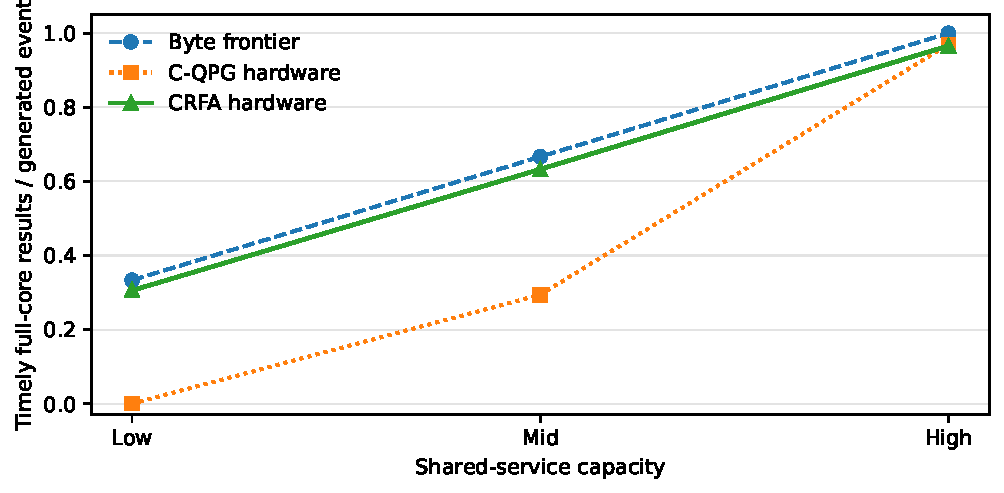
\includegraphics[width=0.82\textwidth]{fig5_crfa_frontier_attainment.pdf}
\caption{Physical timely full-core output relative to the unrestricted
one-round byte frontier. \CRFA{} approaches the byte frontier at all three
capacities, while C-QPG intentionally reserves capacity for per-round remote
coverage at low and mid capacity.}
\label{fig:crfa}
\end{figure*}

At mid capacity, \CRFA{} produces 2,050 timely full-core results from 3,240
generated events, versus 952 under the matched C-QPG sessions. The paired
difference is $+0.3389$ with 95\% session-bootstrap interval
$[0.3306,0.3478]$. At low capacity, C-QPG deliberately sends summaries only,
whereas \CRFA{} yields 0.3056 timely full results per generated event. At high
capacity, both methods admit full evidence for every event; their paired
mean difference is small and the descriptive interval spans zero:
\CRFA{}--C-QPG is $-0.0037$ with interval $[-0.0133,0.0046]$.

These comparisons do not imply that \CRFA{} dominates C-QPG. \CRFA{} obtains
the extra full-evidence slots by assigning no remote evidence to the
non-selected probes in a given round. The primary result is therefore a
measured price of universal per-round coverage, not a generic ranking of
controllers.

\paragraph{Fixed-full overload validation.}
For hardware method C, Proposition~\ref{prop:overload} predicts per-probe
queue growth over 95 generation rounds. The low- and mid-capacity predictions
are 7.9167 and 3.9583~MiB, while sampled hardware maxima are approximately
7.9167 and 3.9584~MiB. At high capacity, $C=3B$ and deterministic overload
disappears. The hardware campaign therefore validates both the feasible side
of the byte boundary and the linear-growth consequence of violating the
long-run load condition.

\subsection{RQ2: Synchronization, Rate Balance, and Timely-Full Efficiency}
At mid capacity, every physical \IQPG{} arm contains exactly 135 \Hfull{}
and 135 \Hnone{} measured actions. The core-required fraction is therefore
$1/2$, and none of those full requests meets the 1-s post-release SLO. The
pattern in Fig.~\ref{fig:cycle} follows Proposition~\ref{prop:cycle}: a synchronized full round
leaves about 43,691~B of queue per probe, far above the largest positive-
payload $v=1$ threshold (about 260.4~B), forcing a synchronized zero-payload
round before the state resets.

\begin{figure}[t]
\centering
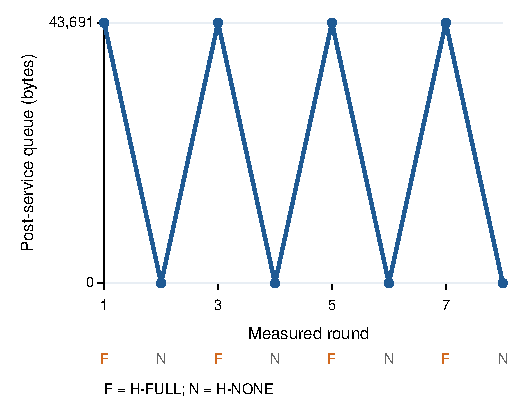
\includegraphics[width=\columnwidth]{fig3_iqpg_cycle_compact.pdf}
\caption{Mechanism detail: the first eight rounds of the archived frozen
$v=1$ mid-capacity I-QPG replay. Full requests (F) leave residual queues;
no-upload actions (N) drain them. The complete 16-round trace is retained
in the Supplementary Extended Mechanism Trace.}
\label{fig:cycle}
\end{figure}

The 12-value sweep in Fig.~\ref{fig:vsweep} reproduces all 36 physical D
session-capacity cells at $v=1$. The mid-capacity core-required fraction
remains exactly $1/2$ through $v=30{,}000$ and becomes 0.6222 only at
$v=100{,}000$; high capacity remains full evidence at every tested $v$.
Low-capacity action composition changes with $v$, so no all-$v$ cycle identity
is claimed.

\begin{figure*}[t]
\centering
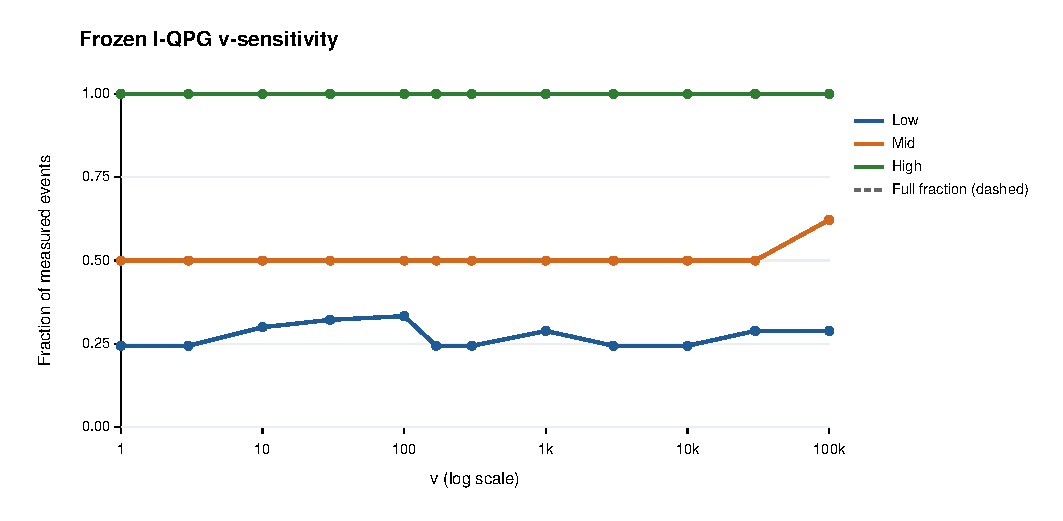
\includegraphics[width=0.92\textwidth]{fig4_v_sensitivity.pdf}
\caption{Parameter robustness: frozen-selector sensitivity across the 12
tested queue weights. Unlike the time-domain mechanism in
Fig.~\ref{fig:cycle}, this sweep tests how behavior changes with $v$.}
\label{fig:vsweep}
\end{figure*}

Phase randomization changes only the probes' initial phases. In this software
study, the desynchronized controller uses only \Hfull{} and \Hnone{}, and
its full-request fractions are exactly $1/3$, $2/3$, and $1$ at low, mid, and
high capacity. These values match Proposition~\ref{prop:prho} with
$p^\star=\rho$, providing conformance to the saturated reduced-regime
prediction rather than evidence that every decentralized controller has that
rate.

The common-denominator mid-capacity software comparison is still useful
because it separates request rate from deadline attainment.
Table~\ref{tab:rq2common} divides timely full-core results by all 270
generated events per simulated arm. C-QPG and the desynchronized independent
controller produce 0.3333 and 0.3352 timely full results per generated event,
respectively, yet C-QPG generates only 14.746~MB versus 23.593~MB---a
37.5\% reduction in application bytes. The synchronized controller generates
17.695~MB but produces no timely full-core result.

\begin{table}[t]
\centering
\caption{Mid-capacity software sensitivity on a common 270-event
denominator. ``Timely full'' is on-time full-core results divided by all
generated events.}
\label{tab:rq2common}
\scriptsize
\begin{tabular}{@{}lrrrr@{}}\toprule
Controller & Full req. & Timely/gen. & Cond. & MB \\
\midrule
C-QPG & 0.333 & 0.3333 & 1.000 & 14.746 \\
Desync. I-QPG & 0.667 & 0.3352 & 0.503 & 23.593 \\
Sync. I-QPG & 0.500 & 0.0000 & 0.000 & 17.695 \\
\bottomrule\end{tabular}

\end{table}

The new hardware extension changes the interpretation of that counterfactual.
At mid capacity, both the phase-randomized independent software policy and
\CRFA{} use a $2/3$ full-request/admission fraction, but their timely output is
very different: 0.3352 in the software phase study versus 0.6327 in the
\CRFA{} hardware extension. This is not a direct hardware-versus-hardware
method comparison, because the phase-randomized policy remains a software
sensitivity. It nevertheless demonstrates why request fraction alone is not a
service result: deterministic joint admission can place work directly on the
same-round feasible frontier, whereas independent queue dynamics can consume
the same long-run byte rate while losing work to deadlines.

C-QPG represents a third operating point. It intentionally gives up one full
slot at mid capacity in exchange for a summary from every probe in every
round. The relevant distinction is therefore among synchronization, deadline
loss, and the security policy of per-round coverage---not a generic
centralized-versus-decentralized ranking.

As a first-order occupancy benchmark, if three probes independently request
full evidence with probability $p=2/3$ in a synchronous slot, then
$P(J=1)=6/27$, $P(J=2)=12/27$, and $P(J=3)=8/27$. With a 2$B$ service budget,
all requests complete within a round for $J\leq2$ but none does for $J=3$
under equal sharing, giving conditional timely fraction $5/9\approx0.556$.
The measured software mean is 0.5028. We treat $5/9$ as an independence
approximation, not a proven upper bound; the gap shows that queue-state
coupling and residual service history matter.

\subsection{RQ3: Physical Hardware Adds Timing Residuals Beyond Byte Feasibility}
The analytical region predicts which payload tuples fit the application
budget; it does not predict OS scheduling, barrier waiting, Wi-Fi timing,
serialization, core execution, or result-return delay.

At high capacity, C, D, E, and F all use \Hfull{} for every measured event.
Mean post-release on-time core-result coverage is 0.9636, 0.9593, 0.9698, and
0.9651, respectively. The paired F--E mean difference is $-0.00463$ with a
descriptive 95\% session-bootstrap interval $[-0.01327,0.00278]$; the F--D
interval also includes zero. Thus, once the byte constraint is non-binding,
the primary hardware data do not show a timing advantage for the
safety-filtered method.

At mid capacity, E and F each admit one full request per three generated
events. Conditional post-release on-time rates among those core-required
events are about 0.8815 and 0.8935. One-round byte feasibility therefore does
not imply perfect physical SLO attainment.

\paragraph{Frontier attenuation in the rotating extension.}
\CRFA{} makes that residual directly measurable because its admitted full
counts equal the analytical unrestricted frontier. Every selected full event
eventually returns a core result at all three capacities, yet the conditional
post-release on-time rates are 0.9167, 0.9491, and 0.9660. Equivalently,
the physical system realizes 91.7\%, 94.9\%, and 96.6\% of the low/mid/high
byte frontier within the 1-s service SLO. Admission opportunities are exactly
balanced across devices: over the 12 sessions each probe receives 360, 720,
and 1,080 full opportunities at low, mid, and high capacity, with maximum
inter-selection intervals of three, two, and one rounds. Timing remains
device-dependent, however. At mid capacity, conditional post-release rates are
0.9153, 0.9319, and 1.0000 for P1, P2, and P3, respectively. Thus, equal
admission opportunity does not imply identical physical deadline attainment.

\paragraph{Schedule-relative release offset.}
Table~\ref{tab:anchors} and Fig.~\ref{fig:timing} aggregate primary-campaign
core-required occurrences by physical probe. P1 and P2 have zero nominal-anchor on-time coverage across
these occurrences, even though their post-release service coverage is
nonzero; P3 retains 0.630 under both anchors. P1's median release offset alone
is about 1.97~s, already larger than the 1-s SLO.

\begin{table}[t]
\centering
\caption{Primary-campaign core-required timing by probe. Coverage is weighted
by core-required event count.}
\label{tab:anchors}
\small
\begin{tabular}{@{}lrrr@{}}\toprule
Probe & Post & Nominal & Lateness p50 (ms) \\
\midrule
P1 & 0.583 & 0.000 & 1972.3 \\
P2 & 0.588 & 0.000 & 763.9 \\
P3 & 0.630 & 0.630 & 83.6 \\
\bottomrule\end{tabular}

\end{table}

The rotating extension reproduces the same anchor asymmetry. P1 and P2
contribute no nominal-on-time full results, whereas P3 is nominally on time
for essentially every selected full event. Consequently, \CRFA{} nominal
timely-full output on the generated-event denominator is only 0.1111, 0.2222,
and 0.3330 at low, mid, and high capacity, compared with post-release values
of 0.3056, 0.6327, and 0.9660.

Source and log inspection identify a mechanism for persistent phase offset:
each probe defines an independent nominal clock before window~0, core submit
forms a three-probe barrier, unequal first-iteration waiting appears
immediately, and each probe subsequently sleeps relative to its completed
iteration rather than catching up to an absolute schedule. The exact OS or
network reason that proposals repeatedly reached the barrier in the observed
P3/P2/P1 order remains unknown.

Crucially, P1's larger nominal release offset is an orchestration-phase
measurement, not evidence that Raspberry Pi~5 computation or inference is
slower. It occurs before the post-release service interval. The primary 1-s
claims are therefore explicitly limited to a \emph{post-release service
SLO}; nominal-anchor results are a schedule-inclusive sensitivity.

\begin{figure*}[t]
\centering
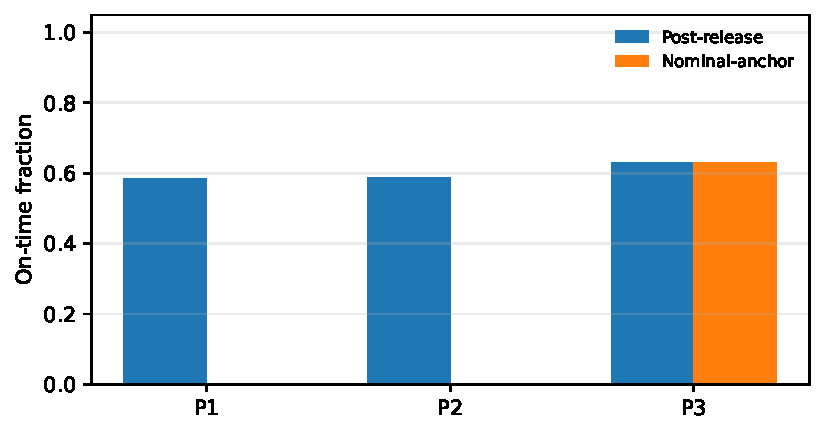
\includegraphics[width=0.92\textwidth]{fig6_timing_anchors_revised.pdf}
\caption{Primary-campaign post-release versus nominal-anchor on-time
coverage, aggregated over core-required occurrences by probe.}
\label{fig:timing}
\end{figure*}

\subsection{RQ4: Scaling Conforms to the Integer Boundary and the Hardware
Result Chain Is Reconstructable}
For the summary-preserving case,
\[
f_n^\star(\rho)=\frac{1}{n}
\left[\left\lfloor n\frac{\rho-\sigma}{1-\sigma}\right\rfloor\right]_0^n,
\qquad \sigma=\frac18.
\]
A discrete-event conformance study evaluates
$n\in\{3,8,16,32\}$ and five normalized capacities. All 20 simulated full
counts match the analytical integer result exactly
(Table~\ref{tab:scale}, Fig.~\ref{fig:scaling}). This is a conformance
check, not physical 32-probe scalability evidence.

\begin{table}[t]
\centering
\caption{Analytical maximum full count $k^\star$ for $m=n$; all 20 values
match the discrete-event conformance simulation.}
\label{tab:scale}
\scriptsize
\begin{tabular}{@{}lrrrrr@{}}
\toprule
$n$ & $\rho=1/3$ & $1/2$ & $2/3$ & $3/4$ & $1$ \\
\midrule
3  & 0 & 1 & 1 & 2 & 3 \\
8  & 1 & 3 & 4 & 5 & 8 \\
16 & 3 & 6 & 9 & 11 & 16 \\
32 & 7 & 13 & 19 & 22 & 32 \\
\bottomrule
\end{tabular}
\end{table}

\begin{figure*}[t]
\centering
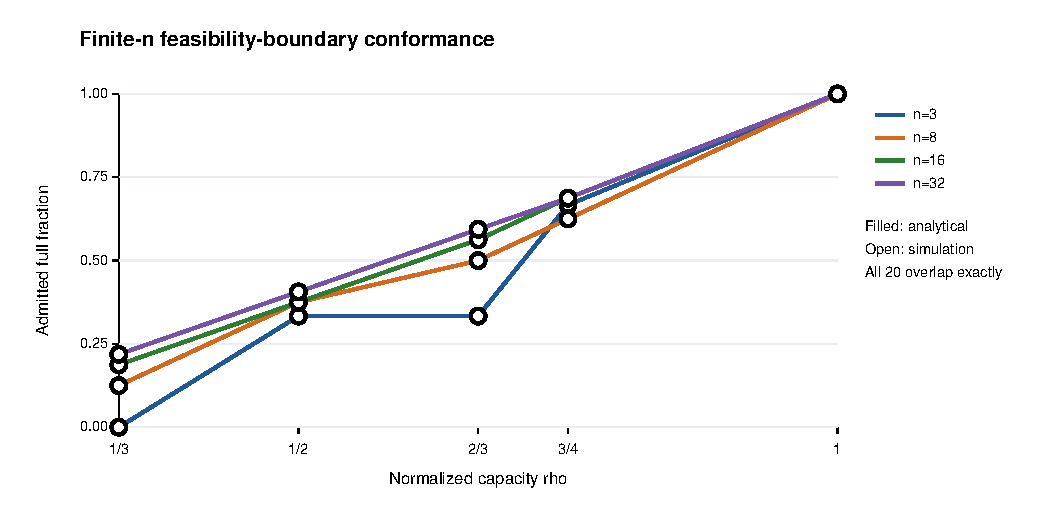
\includegraphics[width=0.92\textwidth]{fig7_scaling_conformance.pdf}
\caption{Discrete-event conformance to the analytical finite-$n$ summary-
preserving boundary.}
\label{fig:scaling}
\end{figure*}

\paragraph{Raw reconstruction.}
The primary full-raw audit rebuilds all 216 accepted hardware arms from
58,320 measured occurrences with zero raw-to-validator/event-metric mismatch
and zero shared-cap violation across 63,720 service rounds. Its verdict
remains \texttt{PASS\_WITH\_ISSUES} because two archival gaps are disclosed:
a direct S03-a01 SSD-failure artifact and S07 pre-hardware launcher-abort
files are absent from the raw bundle. Neither gap changes an accepted arm.

The separately frozen \CRFA{} extension reconstructs 36/36 accepted arms,
9,720 measured occurrences, and 10,620 shared-service rounds. All
event-identity, action/payload-identity, final-drain, reconstruction, and cap
gates pass, with zero shared-cap violations. Its attempt index preserves all
55 attempts, including 19 infrastructure exclusions; timing outcomes were not
used as acceptance gates. Across the two hardware campaigns, 252 accepted arms,
68,040 measured occurrences, and 74,340 reconstructed service rounds are
accounted for, with no shared application-byte cap violation.

The read-only offline analyses contain 432 queue-weight rows, 240 phase-study
rows, 648 primary-campaign timestamp-reconstruction rows, and 20 probe-count
conformance rows, with no retained failed analysis. Only timestamp
reconstruction is derived from measured hardware timestamps; the queue-weight,
phase, and probe-count studies are replay/simulation evidence. The \CRFA{}
timing reconstruction is separately derived from its 9,720 accepted hardware
occurrences.

\paragraph{Role of the safety filter.}
The safety-filtered method records 3,240 \Hfull$\rightarrow$\Hsummary{}
local safety interventions at low capacity, so the path is active. However,
ordinary coordinated admission reaches the same final low-capacity summary
mix. At mid capacity, E and F each record 2,160 full-to-summary capacity
admission degradations, and at high capacity neither mechanism degrades full
evidence. The data support the filter as an auditable local-feasibility
interface, not as an independently superior performance mechanism.

\paragraph{Classifier correctness.}
The formal feature replay yields perfect classification on the scored
occurrences for all frozen detector paths, so correctness adds no information
to the service metric. The dataset is CICIoT2023-derived
~\cite{neto2023ciciot}; the formal occurrence set excludes Recon-PortScan,
and exact feature-vector overlap exists across frozen partitions. In keeping
with long-standing cautions about closed-world IDS evaluation
~\cite{sommer2010closedworld} and recent open-set IIoT work
~\cite{yang2025openset}, we treat detector correctness as a controlled
condition rather than evidence of open-world IDS superiority.

\section{Discussion}
\label{sec:discussion}

\subsection{The Central Trade-off Is Per-Round Coverage versus Timely Richness}
The hardware extension makes the coverage price operational. At mid capacity,
summary-preserving C-QPG spends $2S=32$~KiB on two summaries whenever one
probe receives full evidence. Its timely full-core output is 0.2938 per
generated event. Relaxing same-round universal coverage lets \CRFA{} admit
two full uploads and produce 0.6327. The paired increase, 0.3389 with
descriptive interval $[0.3306,0.3478]$, characterizes this coverage--richness
exchange under the tested workload and nonconcurrent session-matched design.

At low capacity, C-QPG retains universal coarse visibility but no full-evidence
output, whereas \CRFA{} produces 0.3056 timely full results per generated
event. At high capacity, both can admit all three full uploads and the paired
timing interval spans zero. Rotation thus exchanges continuous coarse
visibility for richer evidence over time, with the appropriate operating
point determined by the required representation policy.

\subsection{Synchronization and Admission Are Distinct Mechanisms}
At mid capacity, phase-randomized I-QPG requests full evidence for $2/3$ of
generated events, matching the fraction admitted by \CRFA{}. Within the same software model, however, its timely-full output is only
0.3352. Thus an admissible long-run request rate can coexist with
same-round deadline misses. The physical \CRFA{} measurements separately
quantify how much of a byte-feasible construction meets the hardware SLO.

Synchronized I-QPG additionally suffers phase locking, which creates the
mid-capacity full/none orbit. Coverage reservation, deadline loss, and
synchronization therefore address different design decisions: representation
policy, timely service, and controller phasing.

\subsection{Byte Feasibility Is Necessary but Not Sufficient}
The hardware campaigns measure what byte equations cannot: whether a feasible
upload returns a core result within the service horizon. Every selected
\CRFA{} full result eventually returns, but only 91.7\%, 94.9\%, and 96.6\%
of the low/mid/high byte frontier is realized within the post-release SLO.
The residual is timing, not selected-evidence loss.

Identical opportunity counts likewise do not ensure identical timing. P3 is
essentially always on time after release, whereas P1 and P2 have lower
conditional rates. The primary campaign's schedule-relative phase offset
persists in the extension, separating admission fairness from end-to-end
service fairness.

\subsection{Capacity Planning for Deployment}
\label{sec:deployment}
For universal remote coverage and $k$ full uploads per round, the minimum
one-round byte budget follows directly from Theorem~\ref{thm:frontier}:
\begin{equation}
C_{\min}(k)=nS+k(B-S),\qquad 0\leq k\leq n.
\label{eq:deployment_budget}
\end{equation}
With $n=3$, $B=128$~KiB, and $S=16$~KiB, the 256~KiB middle budget
admits one full upload plus two summaries. Two full uploads with a summary
from the third probe require $2B+S=272$~KiB: an extra 16~KiB, or 6.25\%,
crosses this integer admission threshold. Alternatively, retaining 256~KiB
permits two full uploads under \CRFA{} by assigning no remote upload to the
third probe that round. These are three explicit choices: reserve universal
coverage, increase the budget, or rotate full-evidence coverage. The 272~KiB
threshold is an analytical planning value, not a new hardware configuration
or a physical one-second completion guarantee.

Rotation adds a temporal admission contract: the measured maximum
inter-selection intervals are 3/2/1 rounds at low/mid/high capacity.
Commissioning should check both this opportunity schedule and returned-result
timestamps. A deadline measured from planned release requires the
schedule-inclusive anchor in~\eqref{eq:nomlat}; one measured from actual
event creation uses~\eqref{eq:postlat}. The observed launcher offsets make
this choice consequential even when all admitted bytes fit the budget.

Supplementary Section~IV extends capacity planning to a tolerated downgrade
probability under independent within-round requests and to heterogeneous
summary/upgrade costs. These are analytical planning models, not additional
hardware findings or models fitted to QPG request traces.

\subsection{Evidence Richness Is Not Security Utility}
A summary and a full upload provide different downstream information.
Reducing bytes may improve timeliness while reducing forensic richness;
additional full evidence may increase deadline pressure. Deployment therefore
requires a task-specific value for remote representation and forensic detail,
selected within the measured service-feasibility boundary. Connecting those
values to incident-resolution outcomes is a separate evaluation step.

\section{Limitations}
\label{sec:limitations}

\textbf{Three-probe physical scale.}
The hardware testbed contains three probes. Multi-$n$ results are analytical
and discrete-event conformance checks, not physical validation at 8, 16, or
32 nodes.

\textbf{Rotating extension scope.}
The \CRFA{} extension physically validates one deterministic cyclic
construction at $n=3$; it does not establish optimality over all admission
policies, traffic patterns, or security objectives. Its comparisons with the
primary campaign are matched by frozen session/workload identity but were not
executed concurrently, so paired intervals are descriptive rather than causal
A/B estimates. To preserve session-matched comparability, the extension intentionally
inherited the accepted campaign's service accounting, event schema, timestamp
fields, scoring semantics, and orchestration timing rather than modifying the
launcher; nominal-anchor results therefore remain a schedule-inclusive
sensitivity, and absolute-clock-aligned reruns of both campaigns are left to
future work.

\textbf{Phase randomization is a software sensitivity.}
The desynchronized independent baseline is not a new Pi experiment. It shows
that synchronized failure is not intrinsic to decentralization, but it does
not measure Wi-Fi timing for a physical phase-randomized deployment. Testing
phase offsets as a mitigation without joint admission remains future work.

\textbf{Timing anchor.}
The primary 1-s metric starts at actual event creation. Schedule-inclusive
nominal anchoring is materially stricter: P1 and P2 have zero aggregated
nominal-anchor on-time coverage across the core-required hardware occurrences.
The identified mechanism explains persistence of phase offset, but the exact
OS/network cause of the recurring proposal-arrival order remains unknown.

\textbf{Replay and generalization scope.}
The workload is a frozen CICIoT2023-derived feature replay
~\cite{neto2023ciciot}, not an uncontrolled packet-level deployment.
Recon-PortScan, a major validation-error family, is absent from the formal
replay, and exact feature-vector repetition exists across frozen partitions.
The perfect formal occurrence-level classification therefore does not imply
open-world IDS generalization~\cite{sommer2010closedworld,yang2025openset}.

\textbf{Shield separation.}
The tested campaign does not contain a case where a local device constraint
rejects an action that is independently feasible under the shared network
budget. The safety filter is therefore an implementation/audit interface in
this paper, not an independently proven performance layer.

\textbf{Evidence value.}
The experiment measures coverage, richness, byte demand, and timeliness, not
the downstream incident-resolution value of a summary versus full evidence.
Future work should connect the feasibility region to measured forensic or
cross-probe correlation utility.

\section{Reproducibility and Provenance}
\label{sec:reproducibility}

The primary hardware campaign uses protocol
\texttt{NSF12\_20260906\_RC1}. Accepted scientific attempts are S01-a01,
S02-a01, S03-a02, S04-a02, S05-a01, S06-a01, S07-a02, and S08--S12-a01.
S03-a01, S04-a01, and S07-a01 are invalid infrastructure attempts and are
excluded in full rather than stitched arm-by-arm. The primary full-raw audit
remains \texttt{PASS\_WITH\_ISSUES} only for the two disclosed archival gaps
described in Section~\ref{sec:results}.

The rotating extension uses the separately frozen protocol
\texttt{NSF12\_CRFA\_20260913}. It contains 36 accepted arms from 55 indexed
attempts; 19 infrastructure failures are retained in the attempt index and
excluded in full. Timing outcomes were not acceptance gates. The extension
reconstructs all 9,720 measured occurrences and 10,620 service rounds, with
all event/action/payload/drain/cap gates passing. Frozen markers for the
original 216-arm campaign were checked unchanged before and after the
extension.

The primary campaign, extension, raw audits, and read-only offline analyses
are hashed separately. Offline sensitivity and conformance analyses do not
modify accepted hardware evidence. The artifact package records that the
\CRFA{} mirror resides on the same user-authorized external physical volume
as its primary copy and is therefore an integrity-checked mirror rather than
an independent physical backup. Before public release, the final artifact
will expose persistent checksums and a durable archival identifier. Dataset
redistribution rights are handled separately; reproducibility does not require
redistributing third-party CICIoT2023 content~\cite{neto2023ciciot}.

\section{Conclusion}
\label{sec:conclusion}

\NetShield{} characterizes evidence service under a shared bottleneck through
the one-round region $kB+(m-k)S\leq C$, its unrestricted full-evidence
frontier, and distinct finite-deadline and long-run load conditions. Requiring
universal per-round remote coverage costs one full-evidence slot at low and
mid capacity in the three-probe system, but none at high capacity.

The cyclic hardware construction attains 91.7\%, 94.9\%, and 96.6\% of the
low/mid/high byte frontier. At mid capacity, timely full-core output rises
from 0.2938 under session-matched C-QPG to 0.6327 under \CRFA{}, with paired
difference $+0.3389$ and descriptive 95\% session-bootstrap interval
$[0.3306,0.3478]$, quantifying the exchange from universal per-round
coverage to rotating full-evidence opportunities. Synchronized queue
feedback creates a separate
full/none limit cycle; the phase-randomized software study conforms to the
conditional rate-balance prediction without guaranteeing timely completion.

Every selected \CRFA{} full result is eventually returned, so its gap to the
byte frontier is timing rather than selected-evidence loss. Schedule-relative
release offsets further separate post-release service from nominal deadlines.
Across 252 accepted hardware arms, 68,040 measured events and 74,340
reconstructed service rounds are accounted for with zero shared
application-byte cap violations. Together, the analysis, constructive
controller, and auditable hardware measurements expose which evidence
allocations are feasible and how closely physical service realizes them.

% ============================================================
\begin{thebibliography}{99}

\bibitem{shisher2024timely}
M. K. C. Shisher, Y. Sun, and I.-H. Hou,
``Timely communications for remote inference,'' \emph{IEEE/ACM Trans. Netw.},
vol. 32, no. 5, pp. 3824--3839, 2024,
doi: 10.1109/TNET.2024.3408673.

\bibitem{ari2026goal}
C. Ar\i, M. K. C. Shisher, Y. Sun, and E. Uysal,
``Goal-oriented status updating for real-time remote inference over networks
with two-way delay,'' \emph{IEEE Trans. Netw.}, vol. 34, pp. 4011--4025,
2026, doi: 10.1109/TON.2026.3670099.

\bibitem{zhao2024cur}
Y. Zhao, C. Qiu, X. Shi, X. Wang, D. Niyato, and V. C. M. Leung,
``Cur-CoEdge: Curiosity-driven collaborative request scheduling in edge-cloud
systems,'' in \emph{Proc. IEEE INFOCOM}, 2024, pp. 411--420,
doi: 10.1109/INFOCOM52122.2024.10621190.

\bibitem{hao2024edgetimer}
Y. Hao, S. Yang, F. Li, Y. Zhang, S. Wang, and X. Ren,
``EdgeTimer: Adaptive multi-timescale scheduling in mobile edge computing with
deep reinforcement learning,'' in \emph{Proc. IEEE INFOCOM}, 2024,
pp. 671--680, doi: 10.1109/INFOCOM52122.2024.10621305.

\bibitem{li2025oacr2}
F. Li, Y. Hao, S. Yang, and P. Zhao,
``OACR$^2$: Online admission control and resource reservation for 5G slice
networks with deep reinforcement learning,'' \emph{IEEE Trans. Mobile
Comput.}, vol. 24, no. 8, pp. 7360--7376, 2025,
doi: 10.1109/TMC.2025.3548767.

\bibitem{mirnajafizadeh2024isdc}
S. M. M. Mirnajafizadeh, A. R. Sethuram, D. Mohaisen, D. Nyang, and R. Jang,
``Enhancing network attack detection with distributed and in-network data
collection system,'' in \emph{Proc. 33rd USENIX Security Symp.}, 2024,
pp. 5161--5178.

\bibitem{oqaily2024chainpatrol}
M. Oqaily, H. Purohit, Y. Jarraya, L. Wang, B. Nour, M. Pourzandi, and
M. Debbabi, ``ChainPatrol: Balancing attack detection and classification with
performance overhead for service function chains using virtual trailers,'' in
\emph{Proc. 33rd USENIX Security Symp.}, 2024, pp. 3441--3458.

\bibitem{raza2013svelte}
S. Raza, L. Wallgren, and T. Voigt,
``SVELTE: Real-time intrusion detection in the Internet of Things,''
\emph{Ad Hoc Networks}, vol. 11, no. 8, pp. 2661--2674, 2013.

\bibitem{miettinen2017iotsentinel}
M. Miettinen, S. Marchal, I. Hafeez, N. Asokan, A.-R. Sadeghi, and S. Tarkoma,
``IoT Sentinel: Automated device-type identification for security enforcement
in IoT,'' in \emph{Proc. IEEE ICDCS}, 2017, pp. 2177--2184.

\bibitem{meidan2018nbaiot}
Y. Meidan \emph{et al.}, ``N-BaIoT---Network-based detection of IoT botnet
attacks using deep autoencoders,'' \emph{IEEE Pervasive Computing}, vol. 17,
no. 3, pp. 12--22, 2018.

\bibitem{mirsky2018kitsune}
Y. Mirsky, T. Doitshman, Y. Elovici, and A. Shabtai,
``Kitsune: An ensemble of autoencoders for online network intrusion
detection,'' in \emph{Proc. NDSS}, 2018.

\bibitem{yang2025openset}
X. Yang, F. Tong, F. Jiang, and G. Cheng,
``A lightweight and dynamic open-set intrusion detection for Industrial
Internet of Things,'' \emph{IEEE Trans. Inf. Forensics Security}, vol. 20,
pp. 2930--2943, 2025, doi: 10.1109/TIFS.2025.3546849.

\bibitem{sommer2010closedworld}
R. Sommer and V. Paxson, ``Outside the closed world: On using machine learning
for network intrusion detection,'' in \emph{Proc. IEEE Symp. Security and
Privacy}, 2010, pp. 305--316, doi: 10.1109/SP.2010.25.

\bibitem{mao2017mec}
Y. Mao, C. You, J. Zhang, K. Huang, and K. B. Letaief,
``A survey on mobile edge computing: The communication perspective,''
\emph{IEEE Commun. Surveys Tuts.}, vol. 19, no. 4, pp. 2322--2358, 2017.

\bibitem{mach2017mec}
P. Mach and Z. Becvar, ``Mobile edge computing: A survey on architecture and
computation offloading,'' \emph{IEEE Commun. Surveys Tuts.}, vol. 19, no. 3,
pp. 1628--1656, 2017.

\bibitem{demers1989fair}
A. Demers, S. Keshav, and S. Shenker,
``Analysis and simulation of a fair queueing algorithm,'' in
\emph{Proc. ACM SIGCOMM}, 1989, pp. 1--12.

\bibitem{parekh1993gps}
A. K. Parekh and R. G. Gallager,
``A generalized processor sharing approach to flow control in integrated
services networks: The single-node case,'' \emph{IEEE/ACM Trans. Netw.},
vol. 1, no. 3, pp. 344--357, 1993.

\bibitem{zhang2021emp}
X. Zhang, A. Zhang, J. Sun, X. Zhu, Y. E. Guo, F. Qian, and Z. M. Mao,
``EMP: Edge-assisted multi-vehicle perception,'' in \emph{Proc. 27th ACM
MobiCom}, 2021, pp. 545--558, doi: 10.1145/3447993.3483242.

\bibitem{zhu2024harbor}
R. Zhu, X. Zhu, A. Zhang, X. Zhang, J. Sun, F. Qian, H. Qiu,
Z. M. Mao, and M. Lee, ``Boosting collaborative vehicular perception on the
edge with vehicle-to-vehicle communication,'' in \emph{Proc. ACM SenSys},
2024, pp. 141--154, doi: 10.1145/3666025.3699328.

\bibitem{nishio2019fedcs}
T. Nishio and R. Yonetani, ``Client selection for federated learning with
heterogeneous resources in mobile edge,'' in \emph{Proc. IEEE ICC}, 2019,
pp. 1--7, doi: 10.1109/ICC.2019.8761315.

\bibitem{tassiulas1992}
L. Tassiulas and A. Ephremides,
``Stability properties of constrained queueing systems and scheduling policies
for maximum throughput in multihop radio networks,'' \emph{IEEE Trans.
Autom. Control}, vol. 37, no. 12, pp. 1936--1948, 1992.

\bibitem{neely2010}
M. J. Neely, \emph{Stochastic Network Optimization with Application to
Communication and Queueing Systems}. Morgan \& Claypool, 2010.

\bibitem{huang2024lyapunovbandit}
J. Huang, L. Golubchik, and L. Huang,
``When Lyapunov drift based queue scheduling meets adversarial bandit
learning,'' \emph{IEEE/ACM Trans. Netw.}, vol. 32, no. 4, pp. 3034--3044,
2024, doi: 10.1109/TNET.2024.3374755.

\bibitem{crankshaw2017clipper}
D. Crankshaw, X. Wang, G. Zhou, M. J. Franklin, J. E. Gonzalez, and I. Stoica,
``Clipper: A low-latency online prediction serving system,'' in
\emph{Proc. 14th USENIX NSDI}, 2017, pp. 613--627.

\balance
\bibitem{shen2019nexus}
H. Shen, L. Chen, Y. Jin, L. Zhao, B. Kong, M. Philipose, A. Krishnamurthy,
and R. Sundaram, ``Nexus: A GPU cluster engine for accelerating DNN-based
video analysis,'' in \emph{Proc. 27th ACM SOSP}, 2019, pp. 322--337.

\bibitem{gujarati2020clockwork}
A. Gujarati, R. Karimi, S. Alzayat, W. Hao, A. Kaufmann, Y. Vigfusson, and
J. Mace, ``Serving DNNs like Clockwork: Performance predictability from the
bottom up,'' in \emph{Proc. 14th USENIX OSDI}, 2020, pp. 443--462.

\bibitem{crankshaw2020inferline}
D. Crankshaw, G.-E. Sela, X. Mo, C. Zumar, I. Stoica, J. E. Gonzalez, and
A. Tumanov, ``InferLine: Latency-aware provisioning and scaling for prediction
serving pipelines,'' in \emph{Proc. ACM SoCC}, 2020, pp. 477--491.

\bibitem{khare2025superserve}
A. Khare, D. Garg, S. Kalra, S. Grandhi, I. Stoica, and A. Tumanov,
``SuperServe: Fine-grained inference serving for unpredictable workloads,'' in
\emph{Proc. 22nd USENIX NSDI}, 2025, pp. 739--758.

\bibitem{kadota2019aoi}
I. Kadota, A. Sinha, and E. Modiano, ``Scheduling algorithms for optimizing
age of information in wireless networks with throughput constraints,''
\emph{IEEE/ACM Trans. Netw.}, vol. 27, no. 4, pp. 1359--1372, 2019,
doi: 10.1109/TNET.2019.2918736.

\bibitem{hou2009qos}
I.-H. Hou, V. Borkar, and P. R. Kumar, ``A theory of QoS for wireless,''
in \emph{Proc. IEEE INFOCOM}, 2009, pp. 486--494,
doi: 10.1109/INFCOM.2009.5061954.

\bibitem{baruah1990feasibility}
S. K. Baruah, L. E. Rosier, and R. R. Howell, ``Algorithms and complexity
concerning the preemptive scheduling of periodic, real-time tasks on one
processor,'' \emph{Real-Time Syst.}, vol. 2, pp. 301--324, 1990,
doi: 10.1007/BF01995675.

\bibitem{alshiekh2018shielding}
M. Alshiekh \emph{et al.}, ``Safe reinforcement learning via shielding,'' in
\emph{Proc. AAAI}, 2018, pp. 2669--2678.

\bibitem{wabersich2021filter}
K. P. Wabersich and M. N. Zeilinger,
``A predictive safety filter for learning-based control of constrained
nonlinear dynamical systems,'' \emph{Automatica}, vol. 129, Art. no. 109597,
2021.

\bibitem{ouyang2026sok}
N. Ouyang, A. Shatte, Z. Lu, C. Chen, and W. Xiang,
``SoK: Telemetry-aware runtime assurance for always-on on-device intrusion
detection,'' in \emph{Information Security and Privacy (ACISP 2026)},
LNCS 16794, Springer, 2026, pp. 163--183.

\bibitem{neto2023ciciot}
E. C. P. Neto, S. Dadkhah, R. Ferreira, A. Zohourian, R. Lu, and A. A. Ghorbani,
``CICIoT2023: A real-time dataset and benchmark for large-scale attacks in IoT
environment,'' \emph{Sensors}, vol. 23, no. 13, Art. no. 5941, 2023,
doi: 10.3390/s23135941.

\end{thebibliography}

\end{document}